\part{Description du plastique}
\setcounter{section}{0}
\section{Caract\'eristiques chimiques}
\par{
La mati\`ere de base du plastique est un polym\`ere. On peut classer les polym\`eres selon qu'ils sont naturels provenant du r\`egne animal ou v\'eg\'etal comme la cellulose ou le caoutchouc ou artificiels, obtenus par transformation chimique de polym\`eres naturels ou encore synth\'etiques obtenus par polym\'erisation de monom\`eres. Les polym\`eres sont un  syst\`eme form\'e par un ensemble de macromol\'ecules, entit\'es mol\'eculaires de grande taille issues de l'assemblage covalent d'un grand nombre d'unit\'es monom\`eres r\'ep\'etitives. Les macromol\'ecules ainsi form\'ees, plus grandes que les mol\'ecules simples, apporte au polym\`ere de nouvelles propri\'et\'es, comme la viscosit\'e ou la r\'esistance, que l'on pourra utiliser dans la fabrication de nombreux produits. Le nombre d'unit\'es monom\`eres qui constitue le polym\`ere est appel\'e le degr\'e de polym\'erisation. La masse molaire du polym\`ere est donc directement li\'ee au degr\'e de polym\'erisation. Les polym\`eres synth\'etiques sont donc issus de la polym\'erisation {\citep{fontanille2014chimie}}.
}

\begin{figure}[h]
\centering
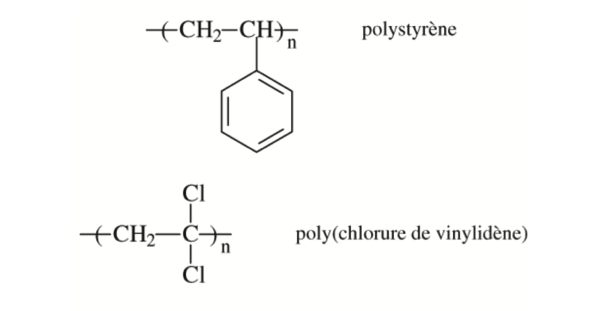
\includegraphics[scale=0.8]{Structurepoly.png}
\caption{Exemples de structure chimique de compos\'es polym\`eres. {\citep{fontanille2014chimie}}} 
\label{structurepoly}
\end{figure}
\FloatBarrier
\par{
Les polym�res peuvent �tre class�s selon leur structure et peuvent pr�senter des architectures lin�aires, ramifi�es ou r�ticul�es. Les polym�res peuvent �tre monodimensionnels et donc lin�aires, r�sultant de la polym�risation des monom�res bivalents.
}

\begin{figure}[h]
\centering
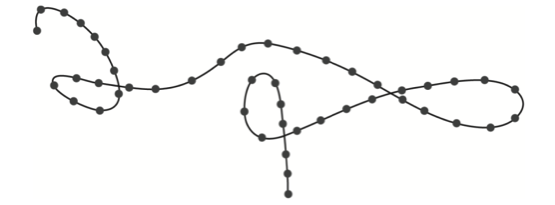
\includegraphics[scale=0.8]{Chainepoly.png}
\caption{Repr\'esentation de a cha\^ine d'un polym\`ere lin\'eaire. {\citep{fontanille2014chimie}}} 
\label{chainepoly}
\end{figure}
\FloatBarrier
\par{
Ils peuvent \'egalement \^etre bidimensionnels essentiellement produits par la nature ou tridimensionnels soit naturels soit r\'esultant de la polym\'erisation de monom\`eres dont la valence est sup\'erieure \`a deux ou encore par r\'eticulation de polym\`eres lin\'eaires par voie chimique ou physique. Leur dimension mol\'eculaire est infinie {\citep{fontanille2014chimie},\citep{Valorplast}}.
}
\begin{figure}[h]
\centering
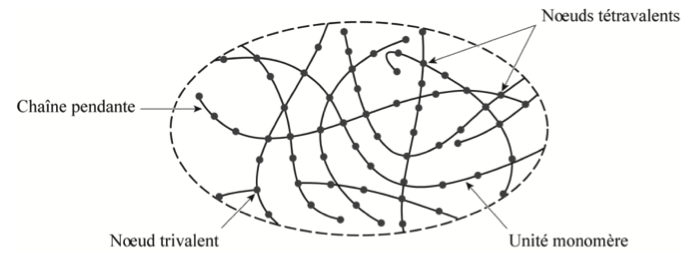
\includegraphics[scale=0.8]{poly3d.png}
\caption{Repr\'esentation sch\'ematique d'un polym\`ere tridimensionnel. {\citep{fontanille2014chimie}}} 
\label{poly3d}
\end{figure}
\FloatBarrier

\par{
La polym\'erisation peut se faire par \'etapes de type polycondensation ou polyaddition comme c'est le cas pour des mol\'ecules lin\'eaires thermoplastiques ou des mol\'ecules r\'eticul\'ees thermodurcissables. La polym\'erisation en cha\^ine est un autre type de r\'eaction de polym\'erisation soit radiculaire, soit ionique comme c'est le cas du polystyr\`ene {\citep{fontanille2014chimie}}. Les plastiques sont rarement utilis\'es tels quels. Les r\'esines sont m\'elang\'ees avec d'autres mat\'eriaux appel\'es "additifs" pour modifier ou am\'eliorer leurs propri\'et\'es et donc leur performance. Ceux-ci peuvent comprendre des charges inorganiques pour renforcer la mati\`ere plastique, des stabilisants thermiques pour permettre le traitement des mati\`eres plastiques \`a des temp\'eratures \'elev\'ees, des plastifiants pour rendre le mat\'eriau flexible et souple, des ignifugeants pour \'eviter la combustion, ainsi que des protecteurs solaire pour \'eviter la d\'egradation lorsqu'ils sont expos\'es \`a la lumi\`ere du soleil. D'autres produits ou colorants peuvent \'egalement \^etre utilis\'es pour am\'eliorer l'aspect du plastique {\citep{andrady2009applications}}.
}

\section{Caract\'eristiques physiques}
\par{
Caract�ristiques physiques
Les polym�res sont dits thermoplastiques, c'est-�-dire qu'� l'�tat fondu, le polym�re devient mall�able ce qui permet de les mouler {\citep{Plasticseurope}}. Ainsi, les polym�res sont durs et rigides � temp�rature ambiante : c'est l'�tat vitreux et sont mous et flexibles � une certaine temp�rature qui est propre aux diff�rents polym�res g�n�ralement autour de 120�C. Il existe une temp�rature de transition vitreuse. Les polym�res thermodurcissables �tant r�ticul�s, l'augmentation de la temp�rature ne permet pas de rompre, de mani�re r�versible, les liaisons covalentes qui les relient car les liaisons des cha�nes primaires se briseraient aussi. Il n'est donc pas possible de les ramollir en �levant la temp�rature. Les polym�res sont �galement class�s selon qu'ils sont cristallins, semi-cristallins ou amorphes {\citep{lecomte2009physique}}.
}